\documentclass[a4paper,12pt]{article}

\usepackage[utf8]{inputenc}
\usepackage[T1]{fontenc}
\usepackage{amsmath}
\usepackage{amssymb}
\usepackage{graphicx}
\usepackage{hyperref}
\usepackage{geometry}
\usepackage[italian]{babel}
\usepackage{svg}
\usepackage{float}
\usepackage{enumitem}

\geometry{a4paper, margin=1in}



\title{Progetto di Algoritmi e Protocolli per la Sicurezza}
\author{Davide D'Acunto\quad Noemi Biancamano}
\date{Gruppo 9}
\begin{document}

\maketitle

\tableofcontents
\newpage
\section{WP 1: Modello}
La seguente sezione si occupa di descrivere gli attori onesti presenti nel sistema, evidenziando le attività che sono interessati a svolgere.
\newline Successivamente, si procede alla discussione degli avversari e del threat model considerato, andando a specificare le capacità e le risorse da essi possedute. Infine, si presentano le proprietà che devono essere preservate dal sistema al fine di essere resiliente agli attacchi considerati.
\subsection{Attori \& Obiettivi}
\begin{figure}[H]
    \centering
    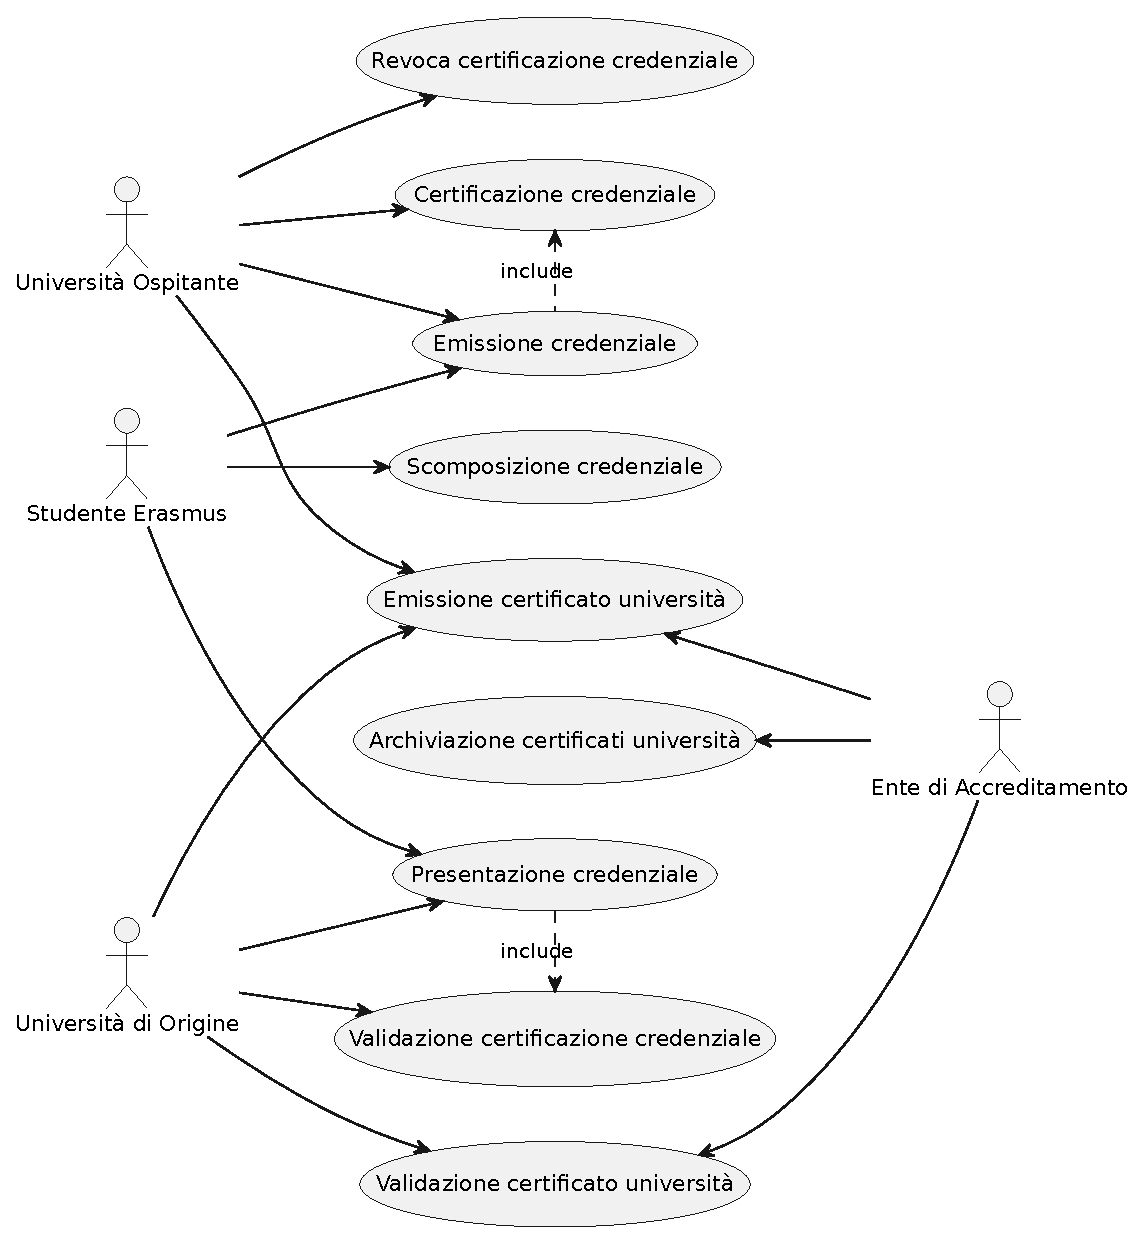
\includegraphics[width=0.95\textwidth]{usecase_1.eps}
    \caption{Use Case degli attori onesti}
    \label{fig:usecase1}
    
\end{figure}
\subsubsection{Studente Erasmus}
Lo studente Erasmus è interessato a sostenere attività accademiche all'interno della sede ospitante, le quali devono essere poi certificate e dimostrate all'università di origine.
\paragraph{Richiesta credenziale} Lo studente deve ricevere dall'università ospitante una credenziale accademica, che attesti le attività da egli effettuate durante il periodo di mobilità.
\paragraph{Trasmissione credenziale} Tale credenziale dev'essere successivamente fornita all'università di origine per certificare le attività svolte dallo studente nella sede ospitante. 
\paragraph{Condivisione selettiva} Lo studente potrebbe desiderare di comunicare solamente un sottoinsieme strettamente necessario delle informazioni contenute all'interno della credenziale, in maniera tale da dimostrare il rispetto dei criteri dell'accordo di mobilità e non rivelare informazioni personali superflue.
\\[0.5em] Si suppone che le risorse computazionali dello studente siano limitate. 

\subsubsection{Università Ospitante}
L'università ospitante, accordatasi con l'università di origine, permette a vari studenti Erasmus di poter usufruire di un periodo di mobilità all'interno della sua sede, nel quale gli studenti hanno la possibilità di effettuare varie attività accademiche.
\paragraph{Emissione credenziale} La sede è interessata a certificare, per ogni studente in mobilità da essa, le attività svolte da questo attraverso una credenziale, cosicché egli sia in grado di comunicarle successivamente alla sua sede d'origine.
\paragraph{Interoperabilità credenziale} Siccome l'università ospitante non conosce i criteri definiti dall'accordo di mobilità per ciascuno degli studenti, inserisce nelle credenziali tutte le informazioni relative alle attività accademiche dello studente, sicché sia poi in grado di poterle comunicare all'università di origine. Tutte le informazioni devono essere rappresentate in un formato standard, definito congiuntamente con l'università di origine, per garantire l'interoperabilità delle credenziali.
\paragraph{Certificazione credenziale} L'ateneo desidera dimostrare che la credenziale è stata effettivamente emessa da sé, per cui rilascia un certificato dell'avvenuta emissione.
\paragraph{Revoca certificazione} In particolari casi laddove si verifichino: errori amministrativi, lo studente fornisce dati fraudolenti, commette plagio, oppure frode, e altre situazioni simili, l'università ospitante deve essere in grado d'invalidare la credenziale revocandone il certificato.
\paragraph{Certificato pubblico} L'università ospitante deve contattare un ente di accreditamento per richiedere un certificato, il quale attesti l'autenticità delle sue comunicazioni, e le permetta di rilasciare certificazioni valide.
% \\[0.5em]Si suppone che le università ospitanti possiedano medie o elevate risorse computazionali.

\subsubsection{Università di Origine}
L'università di origine è accordata con l'università ospitante, mentre con lo studente attraverso un accordo di mobilità. All'interno di questo vengono definite tutte le attività accademiche che allo studente è richiesto soddisfare per validare il suo periodo di mobilità.
\paragraph{Presentazione credenziale} L'ateneo si aspetta di ricevere, da ciascuno studente che ha terminato il proprio periodo di mobilità, una credenziale nella quale sono presenti almeno le attività definite dall'accordo di mobilità.
\paragraph{Validazione credenziale} La credenziale deve essere certificata dall'università ospitante, cosicché si abbia la certezza della validità di questa. Qualora la credenziale non fosse certificata, invalida oppure revocata, l'ateneo è in grado di rifiutare la credenziale.
\paragraph{Verifica certificato} L'università di origine deve poter verificare l'autenticità della credenziale, attraverso la verifica del certificato associato a essa.

\subsubsection{Ente di accreditamento}
L'ente di accreditamento è un'autorità esterna, che si occupa di certificare le università, in modo tale da garantire l'autenticità delle comunicazioni. 
\paragraph{Emissione certificato} L'ente di accreditamento emette certificati per le università che lo richiedono, i quali vengono utilizzati da queste per certificare o validare credenziali.
\paragraph{Archiviazione certificati} Non solo, si occupa anche dell'archiviazione delle certificazioni associate alle università, conservandole sino a una determinata data, e rendendoli disponibili per la validazione.
\paragraph{Revoca certificato} L'ente di accreditamento deve essere in grado di revocare i certificati emessi, qualora vi siano errori o violazioni.

\subsection{Credenziale}
La credenziale è un documento contenente le informazioni relative alle attività accademiche che lo studente in mobilità ha svolto nella sede ospitante. 
\newline Le informazioni contenute all'interno della credenziale sono le seguenti:
\begin{itemize}
    \item Matricola interna dello studente
    \item Nome e cognome dello studente
    \item Matricola esterna dello studente
    \item Codice e nome dell'università ospitante
    \item Nome e cognome del referente dell'università di origine
    \item Nome e cognome del referente dell'università ospitante
    \item Data di emissione  
    \item Data di fine validità
    \item Periodo di mobilità
    \item Per ciascun esame sostenuto:
    \begin{itemize}[label=$\circ$]
        \item Nome e codice dell'esame
        \item Eventuale voto espresso in trentesimi, oppure esito
        \item Eventuale lode
        \item CFU conseguiti
        \item Data di superamento dell'esame
        \item Nome e cognome del docente
        \item Nome e codice del corso di laurea
    \end{itemize}
    \item Per ciascuna attività svolta:
    \begin{itemize}[label=$\circ$]
        \item Nome e codice dell'attività
        \item Periodo d'inizio e fine dell'attività
        \item Eventuali CFU dell'attività
        \item Nome e cognome del docente o del referente
    \end{itemize}
\end{itemize}
Le università devono attenersi a questo formato per assicurare l'interoperabilità delle credenziali emesse.
\subsection{Threat Model}
Come threat model si considerano avversari che potrebbero compromettere il sistema con una determinata sequenza di azioni, le quali dipendono dalle risorse e capacità da essi possedute, definendo poi quale sia la proprietà che potrebbe venire meno laddove il sistema non sia resiliente a tale attacco.
\newline Ciascun attaccante viene considerato efficiente e probabilistico, ovvero con una determinata probabilità di avere successo nell'intento in tempo polinomiale.
\subsubsection{Violazione dell'ente di accreditamento}
Si prende in esame il caso in cui l'ente di accreditamento venga compromesso da un attaccante, il quale riesce a ottenere accesso ai meccanismi di emissione e revoca dei certificati. In questo caso, l'attaccante potrebbe emettere certificati falsi, oppure revocare certificati validi.
\newline In questo caso si perde la proprietà di autenticità, in quanto non si ha la certezza che il certificato sia stato emesso da un'autorità competente, problema che si ripercuote sulle comunicazioni tra gli altri attori, siccome la loro fiducia nella sicurezza si basa sui certificati emessi.
\subsubsection{Violazione dell'università ospitante}
Si considera lo scenario dove l'università ospitante viene compromessa da un attaccante, il quale riesce a ottenere accesso ai meccanismi di emissione, certificazione e revoca delle credenziali. In questo caso, l'attaccante diverrebbe in grado di:
\begin{itemize}
    \item Emettere credenziali false
    \item Certificare credenziali false
    \item Revocare certificazioni
\end{itemize}
In questo caso si perde la proprietà di autenticità, siccome non si ha la certezza che la certificazione sia stata emessa dall'università.
\subsubsection{Violazione dell'università di origine}
Si analizza il caso in cui l'università di origine venga compromessa da un attaccante, il quale riesce a ottenere accesso ai meccanismi di validazione delle credenziali. In questo scenario, l'attaccante potrebbe accettare credenziali false, oppure respingere credenziali valide.
\newline Così si perde la proprietà di confidenzialità, poiché l'attaccante sarebbe in grado di accedere a informazioni riservate riguardanti studenti, attraverso le credenziali che inviano all'ateneo, ignari che sia stato violato.
\subsubsection{Studente malevolo}
Si studia il caso laddove lo studente sia malevolo, e tenti di far passare come valida una credenziale insufficiente, oppure alterata. In questo caso, lo studente potrebbe violare la proprietà d'integrità e autenticità della credenziale.
\subsubsection{Intercettatore di comunicazioni dell'università ospitante}
Si prende in esame la presenza di un attaccante che intercetti tutte le comunicazioni da e verso l'università ospitante. Questo attaccante ha accesso a uno storico di messaggi cifrati e relative decifrature attraverso mezzi alternativi. 
\newline In questo caso, l'attaccante potrebbe essere in grado d'inferire informazioni sui successivi messaggi cifrati, violando la proprietà di confidenzialità. Non solo, l'attaccante potrebbe alterare le comunicazioni in uscita, violando quindi le proprietà di sicurezza del sistema.
\subsubsection{Ascoltatore di comunicazioni dello studente}
Si prende in esame la circostanza di un attaccante che ascolti le comunicazioni tra studente e altri attori, presente sul canale di comunicazione prima che questa avvenga. In questo caso, l'attaccante potrebbe carpire informazioni riservate, come la credenziale dello studente, violando la proprietà d'integrità.
\subsubsection{Attacco con credenziale nota}
Si tiene in considerazione il caso di un attaccante che riesca ad ascoltare la conversazione tra l'università di origine e uno studente di cui conosce la credenziale attraverso altri mezzi.
\newline In questo caso, l'attaccante potrebbe inferire informazioni riguardati il meccanismo di comunicazione sicura, e violare le proprietà di sicurezza del sistema. 
\subsubsection{Divulgazione di informazioni superflue}
Si considera lo scenario in cui uno studente divulghi involontariamente più informazioni di quelle necessarie, all'università di origine. Così facendo, lo studente rivelerebbe informazioni riservate, e non approfitterebbe della possibilità di divulgare selettivamente le sole informazioni strettamente necessarie, richieste dall'università. Spesso, questo tipo di evento avviene per errore, o per ignoranza.
\subsection{Proprietà}
In questa sezione si discuteranno con maggior riguardo le proprietà che il sistema deve possedere per soddisfare i requisiti di sicurezza richiesti.
\subsubsection{Confidenzialità}
Con confidenziale si intende l'accesso alle informazioni solamente a coloro che sono autorizzati. Nessun individuo non autorizzato deve accedere, neanche in parte, ad alcuna informazione che non è loro permesso di vedere.
\subsubsection{Integrità}
Con proprietà d'integrità ci si riferisce alla garanzia che non vi siano alterazioni di messaggi durante la trasmissione. 
\subsubsection{Autenticità}
L'autenticità è la proprietà che assicura l'originalità del messaggio, ovvero che sia stato effettivamente inviato dal mittente, e che non ci sia stata alcuna impersonificazione.
\subsubsection{Revocabilità}
La revocabilità è l'abilità da parte di un ente certificatore di revocare una sua certificazione precedentemente emessa. Ciò richiede che l'ente informi tutti gli attori interessati di ciascuna revoca.
\subsubsection{Non ripudio}
La proprietà di non ripudio è la garanzia con la quale un attore non è in grado di negare di aver effettuato una certa azione. In questo caso, l'attore non è in grado di negare di aver emesso una credenziale.
\subsubsection{Interoperabilità}
L'interoperabilità è la proprietà che assicura che le credenziali emesse da un'università siano riconoscibili dalle altre università, a patto che rispettino un formato definito.
\subsubsection{Disponibilità}
La disponibilità è la proprietà che assicura continua operatività del sistema, ovvero che gli attori siano in grado di accedere e utilizzare il sistema in qualsiasi momento.
\subsubsection{Trasparenza}
La trasparenza è la proprietà attraverso la quale ciascun attore è sempre in grado di risalire all'autore di una data azione, possa essa essere l'emissione di un certificato, oppure la sua revoca.
\subsubsection{Scalabilità}
La proprietà di scalabilità garantisce che non vi sia riduzione delle prestazioni del sistema, all'aumentare dei nodi.
\subsubsection{Divulgazione selettiva}
Ciascuno studente deve poter essere in grado di divulgare soltanto un sottoinsieme strettamente necessario delle sue informazioni. Tale proprietà è denominata divulgazione selettiva.



\newpage
\section{WP 2}
\subsection{Introduzione alla soluzione}
In questa sezione si presenta la soluzione proposta per il modello descritto precedentemente.
\newline Nella prima sezione si descrive il sistema di certificazione delle università, il quale permetterà il rispetto della proprietà di autenticità, fondamentale per la parte successiva. In questa parte vengono trattate le interazioni tra le università e l'ente di accreditamento.  
\newline Segue l'esposizione del sistema di gestione dei certificati delle credenziali degli studenti, il quale si basa sull'utilizzo dei certificati per l'autenticazione delle università nel sistema. Le interazioni rappresentate sono quelle tra le università. 
\newline Infine, si spiega come lo studente possa utilizzare il sistema per validare le attività svolte durante il periodo di mobilità. Qui ricadono le interazioni tra lo studente e le università. 
\newline Per ciascuna di queste sezioni, si tengono in considerazione le proprietà di sicurezza precedentemente elencate, sottolineandone i meccanismi progettati per garantirle.
\subsection{Certificati digitali} 
Il meccanismo dei certificati digitali si basa sull'utilizzo della crittografia asimmetrica, che garantisce le proprietà di confidenzialità, integrità e autenticità nelle comunicazioni. 
In questo contesto, l'ente di accreditamento si considera essere un'autorità certificante (CA): quando necessario, l'università contatta la CA per richiedere un certificato.
\newline
Un certificato digitale è un documento elettronico che associa una chiave pubblica a un'identità, e viene firmato digitalmente dalla CA. Nel documento sono presenti informazioni riguardanti l'università e la sua chiave pubblica, la CA e la sua firma, e il periodo di validità del certificato. Il certificato rappresenta una garanzia di affidabilità, in quanto la CA è un ente di fiducia che rende disponibile pubblicamente la chiave pubblica dell'università.
\subsubsection{Emissione certificato} Quando l'università necessita di essere certificata per rendere nota la propria chiave pubblica deve contattare una CA, e fornirle le informazioni necessarie alla creazione del certificato digitale. In particolare, l'università deve generare una coppia di chiavi pubblica e privata, e fornire alla CA la chiave pubblica, più il proprio identificativo. La CA, per garantire che stia effettivamente dialogando con l'università, deve verificarne via mezzi alternativi l'identità, siano essi l'utilizzo di un Identity Provider, canale preesistente sicuro, o di persona. Una volta fatto ciò, emette il certificato digitale associato alla chiave pubblica dell'università, firmandolo con la propria chiave privata.
\subsubsection{Revoca Certificato} Di norma, i certificati hanno una scadenza temporale, dopo la quale non sono più validi, e quando scade, l'università deve rinnovarlo ripetendo la procedura di cui sopra. Tuttavia, in particolari circostanze, la CA potrebbe decidere di revocare un certificato prima che questo scada. Ciò può avvenire quando il certificato è errato, ma anche laddove venisse compromessa la chiave privata dell'università o della CA. In caso di revoca di un certificato, la CA deve informare tutti gli attori interessati, in modo tale che non venga più utilizzato.
\subsubsection{Validazione certificato} Siccome il certificato può essere revocato prima della data di scadenza, è necessario un meccanismo che permetta di valutare se un certificato è valido nel senso che, durante la durata di validità, non è stato revocato. Per permettere ciò, è innanzitutto necessario che la CA archivi i certificati non scaduti, ma revocati. Dopodiché, ogni attore deve accedere, almeno una volta, alla lista dei certificati revocati, siccome altrimenti non sarebbe in grado di sapere se un certificato sia valido o revocato. Per ottimizzare le risorse computazionali e spaziali, gli attori potrebbero, piuttosto che chiedere costantemente alla CA se un certificato sia valido o meno, e renderlo quindi un singolo punto di fallimento, salvare periodicamente in locale una lista dei certificati revocati. Per risparmiare poi ulteriore spazio, è possibile conservare, dei certificati in corso di validità, solamente il loro identificativo, e un bit che ne attesti la validità (Certificate Revocation Vector).
\subsubsection{Punto di fallimento} L'aggiornamento della lista dei certificati revocati deve avvenire periodicamente ed online, cosicché ciascuna università rimanga aggiornata riguardo le revoche e l'autenticità delle comunicazioni, anche in assenza di accesso alla rete.
\newline In questo caso, però, la CA diventerebbe un singolo punto di fallimento, siccome qualora non dovesse essere disponibile, gli attori non sarebbero in grado di ottenere le nuove liste. Per cui si considera l'utilizzo di un insieme di CA, le quali si comportano come singole CA indipendenti ma comunicanti tra loro. Le CA comunicano tra loro le revoche, e ciascuna di esse è in grado di emettere certificati per le università, inoltre, ciascuna di esse è in grado di validare i certificati emessi dalle altre CA. In questo modo si assicura la proprietà di disponibilità, tuttavia diventa necessario gestire più liste di revoche, una per ciascuna CA.
\subsubsection{Gestione delle liste ed aggiornamento} Siccome le università hanno sufficienti risorse per gestire più liste, l'implementazione della gestione di queste non comporta un problema. Rimarrebbe da definire una periodicità di aggiornamento delle liste, ma sarebbe possibile lasciare che siano le CA ad occuparsi di ciò: qualora una CA emetta una revoca, lo comunica immediatamente a tutte le CA e università da essa conosciute, e loro propagano l'informazione, inoltrando il messaggio originale.
\newline L'inoltro del messaggio originale permette la trasparenza del sistema, in quanto ciascuna CA è in grado di sapere chi ha emesso la revoca. Tale informazione ritorna fondamentale nella gestione di eventuali conflitti: siccome le università possiedono più liste, è possibile che una CA emetta una revoca prima delle altre, in tal caso si assume che, con la revoca di un singolo certificato da parte di una CA, la chiave pubblica che vi era associata sia inaffidabile, anche se appare in altri certificati non revocati. La chiave pubblica, associata ad un certificato revocato di un'università, può diventare nuovamente affidabile solamente nel caso in cui altre CA revochino il certificato della CA che l'ha revocata.
\subsubsection{Gerarchia delle CA} Siccome anche il gruppo di CA necessita di chiavi pubbliche affidabili per emettere i certificati e comunicare gli aggiornamenti, è necessario che ciascuna di esse venga certificata da altre CA, in maniera reciproca. In questo modo, si ha una gerarchia di CA, in cui ciascuna CA è in grado di emettere certificati per le università, e ciascuna CA è in grado di validare i certificati emessi dalle altre CA.

\subsection{Sistema di gestione dei certificati delle credenziali}
Per garantire l'accesso pubblico ai certificati delle credenziali è necessario un archivio digitale, condiviso tra le università. Tuttavia da questo non devono trasparire informazioni riservate, siccome non vi sono restrizioni sull'accesso. È quindi necessario non poter inferire, dai certificati emessi dalle università, informazioni sulle credenziali a cui sono associati.

\subsubsection{Certificazione della credenziale}
Quando l'università desidera emettere una certificazione per una credenziale, deve fornire tramite la credenziale, un identificativo univoco, da cui non è possibile dedurre alcuna informazione su essa. 
Tale identificativo è contenuto nella certificazione, permettendo a chiunque la possieda, di validare la credenziale, e corrisponde ad una struttura dati contenente un insieme di digest, ottenuti attraverso l'applicazione di una funzione di hash alle varie parti della credenziale. In particolare nella credenziale le parti a cui viene applicato l'hash sono: 
\begin{itemize}
    \item Le informazioni riguardanti lo studente, le università, la credenziale e il periodo di mobilità 
    \item Ciascun esame e le relative informazioni 
    \item Ciascun attività e le relative informazioni
\end{itemize}
Per cui la struttura dati conterrà: un hash per ciascun esame, un hash per ciascuna attività e un hash per le altre informazioni rimanenti. 
\subsubsection{Merkle Tree}
La struttura dati a cui si è fatto riferimento è un albero, denominato Merkle Tree, le cui proprietà sono: 
\begin{itemize}
    \item Ciascuna foglia contiene l'hash di un blocco di informazioni 
    \item Ciascun nodo interno contiene l'hash della concatenazione del contenuto dei due nodi figli 
    \item L'albero è pieno, ciascun nodo o ha due figli o è un nodo foglia 
\end{itemize}
Queste proprietà garantiscono la possibilità di divulgare le sole informazioni desiderate, permettendo comunque di validarle. 
\subsubsection{Validazione selettiva}
Determinato un Merkle Tree di una credenziale, è possibile effettuare il processo di validazione della credenziale attraverso di esso. Se tutte le informazioni della credenziale sono fornite, calcolando l'hash per ciascun blocco di informazioni, attraverso la stessa procedura che si è precedentemente discussa, si otterrà un insieme di blocchi di hash. Si controlla quindi la presenza di ciascun blocco all'interno delle foglie: se vi è un'associazione uno a uno il Merkle Tree è effettivamente calcolato sulla credenziale. 
\newline Tuttavia, se non tutte le informazioni della credenziale vengono fornite, non è possibile confrontare tutte le foglie, per cui si utilizza la dimostrazione di appartenenza. Si individuano le foglie a cui appartengono gli hash calcolati e si valuta il loro percorso sino alla radice: se ciascun nodo intermedio è correttamente calcolato come l'hash della concatenazione dei nodi figli, allora le informazioni parziali appartengono ad una credenziale valida. 
\subsubsection{Certificazioni \& Blockchain} 
Un'università che desidera emettere una certificazione per una credenziale, ne deve decidere la durata di validità e poi calcolare su essa il Merkle Tree. Ottenuto questo, deve pubblicare il Merkle Tree a tutte le università che potrebbero essere interessate a validare tale credenziale. L'archivio condiviso, dove vengono conservati tutti i Merkle Tree, è una blockchain, dove a ciascun Merkle Tree è inoltre associato l'hash corrispondente alla radice del Merkle Tree precedente, ovvero un puntatore hash al Merkle Tree precedente.
\newline Si considerano il Merkle Tree e il puntatore hash 
appartenenti ad un blocco, nel quale vi è anche l'informazione riguardante la chiave pubblica dell'università che l'ha generato ed un identificativo univoco del blocco, ottenuto attraverso l'hash dell'intera credenziale. 
Da qui si considera certificazione il blocco e il suo contenuto nel suo insieme. 
\newline Con informazione riguardante la chiave pubblica dell'università che ha generato il blocco, si intende una procedura che assicura l'autenticità e il non ripudio del suo contenuto.
Quando l'università genera un blocco, cifra la radice del Merkle Tree mediante la sua chiave privata, e quando successivamente un'università desidera verificarne l'autenticità, decifra quel campo con la chiave pubblica di tale università, e si aspetta di ottenere lo stesso risultato.
\subsubsection{Smart Contract e transazioni}
Per automatizzare e semplificare i processi di caricamento e validazione di una certificazione, si utilizza uno smart contract, il quale rappresenta un'interfaccia standard per le università. Lo smart contract si occupa di generare il blocco a seconda dei dati ricevuti dall'università, quando desidera emettere un certificato, i quali vengono inviati all'interno di un messaggio detto transazione.
\newline Per garantire la proprietà di trasparenza, la transazione è pubblicamente visibile siccome è salvata nella blockchain, all'interno di questa vi sono, informazioni quali: l'indirizzo dell'università nella blockchain, il contenuto della richiesta e l'indirizzo di destinazione, il quale corrisponde a quello del contratto. 
\newline Sempre per trasparenza, sia il codice che lo stato dello smart contract risiedono sulla blockchain, cosicché che tutti i partecipanti ne possano verificare il corretto funzionamento.
\subsubsection{Revoca certificazione}
Riguardo la procedura di revoca di una certificazione, già presente sulla blockchain, lo smart contract mette a disposizione un'interfaccia di comunicazione per la gestione di tale eventualità.
\newline Siccome non è possibile alterare un blocco una volta caricato, poiché renderebbe invalidi i puntatori hash e quindi la catena, si aggiunge allora un nuovo blocco, il quale scopo è quello di invalidare la certificazione. Questo blocco contiene le stesse informazioni contenute in quello della certificazione, più una flag di invalidità posta al valore di vero.
\newline Per assicurare uniformità ai blocchi della catena, anche ai blocchi riguardanti la creazione della certificazione si include questa flag, posta al valore falso.
\newline Le politiche di revoca di una certificazione sono due: 
\begin{itemize}
    \item L'autore della certificazione è automaticamente in grado di revocarla, per cui si aggiunge all'interno di ogni blocco l'indirizzo dell'autore. Il contratto mette a disposizione questa tipologia di revoca.
    \item Un numero sufficiente di università decide di revocare la certificazione, qualora essa non rispetti determinati criteri oppure l'università autrice venga estromessa dal sistema. 
\end{itemize}
Ovviamente, purché sia possibile revocare una certificazione, è necessario che ne si conosca l'ID del blocco che l'ha generata, il quale è univoco per ciascun blocco: lo smart contract utilizza il campo riservato al Merkle Tree per inserire il riferimento all'ID del blocco che viene revocato.
\subsubsection{Meccanismo di validazione}
Siccome generalmente nella blockchain, è il solo smart contract a generare blocchi, si potrebbe non intravedere la necessità della validazione dei blocchi. Tuttavia, tutti i partecipanti sarebbero in grado di generare dei blocchi, per cui è necessaria una procedura attraverso la quale le università siano in grado di decidere quali blocchi debbano essere salvati e quali no. 
\newline Questa procedura richiede che almeno un certo numero, di tutte le università presenti nel sistema, acconsenta all'inserimento di tale blocco nella blockchain. Il numero esatto è un compromesso tra la sicurezza del sistema e la velocità di revoca, ed è fortemente dipendente dal numero di università presenti nel sistema.
\subsection{Studenti ed emissione credenziale}
Gli utenti finali che accedono a questo sistema mediante le università sono gli studenti, i quali non sono consapevoli della blockchain e dei certificati, siccome vi interagiscono indirettamente mediante le università. Le azioni che interessano gli studenti sono: ricezione della credenziale dall'università ospitante, condivisione selettiva delle sole informazioni necessarie all'interno di questa, e l'invio di esse all'ateneo di origine.
\newline Tuttavia, per poter effettuare queste operazioni, è necessario stabilire una comunicazione sicura verso le università, e poi che lo studente si autentichi perché sia garantito che la persona dietro tali azioni sia proprio lui.
\subsubsection{Autenticazione dello studente}
Ciascuno studente deve essere in grado di dimostrare la propria identità all'università ospitante, o a quella di origine, senza tuttavia rivelare il meccanismo sottostante, e mediante l'utilizzo di un dispositivo con scarse risorse computazionali.
\newline Innanzitutto, lo studente deve aprire una prima comunicazione con l'università, la quale possiede un certificato che le associa la propria chiave pubblica: lo studente ottiene il certificato mediante una CA e diventa in grado di comunicare con confidenzialità con l'università. Tuttavia, l'università non è ancora in grado di autenticare lo studente, poiché non possiede alcuna informazione riguardante esso, neanche può comunicare in segretezza con esso, siccome lo studente è sprovvisto di un certificato. Riguardo i certificati, se lo studente non conosce quello relativo alla sua università, può richiederlo a una CA, e conservarselo per le comunicazioni future. Tuttavia, per accertarsi che rimanga aggiornato, lo studente deve periodicamente controllare una eventuale revoca da parte della CA, in rete, siccome è comunque attraverso la rete che comunica con l'università.
\newline Lo studente che desidera autenticarsi per la prima volta deve innanzitutto dimostrare la propria identità, ma successivamente può decidere una chiave di crittografia, con la quale stabilire una comunicazione sicura con l'università durante tale sessione. Una volta che lo studente possiede tale chiave e la comunica all'università, quest'ultima è in grado di cifrare i propri messaggi verso lo studente, che li può decifrare facilmente.
\newline La soluzione al problema di autenticazione è l'invio di un identificativo univoco, come un account email attraverso cui lo studente sia in grado di ricevere messaggi, e successivamente una password, utilizzata come mezzo di autenticazione. Sebbene sia semplice da implementare, questo meccanismo non è sicuro: è necessario affiancare infine a questo un timestamp, e magari anche la risposta a una challenge iniziata dall'università durante la fase di autenticazione.
\newline Per rendere ancora più sicuro questo meccanismo, si potrebbe affiancare alla password anche un autenticatore sul dispositivo dello studente, come un applicazione che genera un codice temporaneo mono uso. Qualora lo studente debba perdere l'autenticatore, deve però identificarsi nuovamente, e può farlo solo recandosi di persona all'università se tale strumento è reso disponibile dall'università. Per ovviare a questo problema, l'università potrebbe anche fare uso di servizi terzi di autenticazione, cosiddetti Identity Provider. Strumenti del genere sono comuni qualora le università appartengano a un consorzio di università, e quindi condividano un Identity Provider comune, il quale permette di autenticare lo studente in maniera sicura.
\newline La decisione finale, nello scambio di messaggi che avviene per l'autenticazione, è che lo studente intenzionato ad autenticarsi invii sia il timestamp del messaggio, che una coppia di numeri casuale. Quando l'università riceve il messaggio, lo decifra e risponde con uno dei numeri casuali inviati precedentemente. In questo modo, lo studente è sicuro che sia l'università ad aver risposto al messaggio, e ne verifica l'autenticità dalla firma, sebbene il messaggio sia in chiaro. Fatto ciò, lo studente invia la propria password cifrandola con la chiave pubblica e allega il secondo nonce. L'università sarà sicura che sia stato lo studente a rispondere, siccome solo lo studente poteva conoscere tale numero casuale. Eventualmente, può anche comunicare la chiave con la quale continuare la comunicazione in maniera sicura, altrimenti l'università può rispondere, ma non può aspettarsi di poter verificare l'effettiva autenticità dei messaggi successivi, se la comunicazione non aggiunge ulteriori nonce casuali.
\newline L'università dovrà conservare le varie associazioni username password, per poter riconoscere dalle credenziali lo studente in futuro. La password non viene salvata in chiaro ma conservata con un hash combinato a un salt univoco per ciascuno studente.
\newline L'utilizzo della chiave simmetrica per la sola sessione è una questione di sicurezza ed efficienza, per alcuni documenti, come la credenziale, la crittografia asimmetrica comporterebbe un rallentamento proporzionale alla quantità d'informazione contenuta nei messaggi, che potrebbe essere alta in caso di foto di documenti. Siccome poi la chiave di sessione è univoca per ciascuna sessione, il rischio di compromissione della chiave viene ridotto.
\subsubsection{Ricezione credenziale}
Una volta che lo studente ha stabilito un canale sicuro con l'università ospitante, è pronto per richiedere la trasmissione della credenziale. L'università ospitante procede generando la credenziale, contenente le informazioni riguardanti le attività dello studente, e la certificazione di questa. Associa alla credenziale una determinata durata di validità, e la cifra con la chiave di sessione, inviandola quindi allo studente. Dopodiché, calcola l'hash sui vari blocchi della credenziale, secondo le modalità precedentemente descritte, e invia una transazione allo smart contract, il quale provvederà a generare un blocco con le informazioni ricevute, e a pubblicarlo nella blockchain.
\subsubsection{Divulgazione selettiva}
Una volta che lo studente ha ricevuto la credenziale, è in grado di decidere quali informazioni divulgare all'università di origine. Il meccanismo di divulgazione selettiva può essere, per semplificare il lavoro dello studente, implementato come un'applicazione offline che, grazie allo standard definito per le credenziali, permetta di selezionare le informazioni da divulgare, e produrre una nuova credenziale, contenente solamente le informazioni selezionate.
\newline Siccome è una semplice scomposizione d'informazioni da un file di testo, basse prestazioni computazionali sono più che sufficienti.
\subsubsection{Trasmissione credenziale}
Una volta che lo studente ha ottenuto la credenziale, ed eventualmente deciso quali informazioni divulgare, è pronto per inviarla all'università di origine. Stabilisce quindi, attraverso la stessa procedura menzionata precedentemente, un canale sicuro con l'ateneo, ottenendo una nuova chiave di sessione. Cifra quindi la credenziale con questa chiave, e la invia ad essa. Subito dopo, l'università calcola blocchi di hash dalla credenziale, e contatta lo smart contract sulla blockchain per richiedere la validazione della credenziale.
\newline In base alle circostanze vi possono essere scenari differenti:
\paragraph{Credenziale certificata} La credenziale è correttamente certificata in un blocco della blockchain, e lo smart contract restituisce l'ID del blocco, il quale è unico per quella credenziale. L'università di origine può quindi procedere a validare la credenziale, e a registrarla nel proprio sistema, qualora le informazioni in esse siano sufficienti.
\paragraph{Credenziale non certificata} Non esiste alcuna certificazione per la credenziale, e lo smart contract restituisce un errore. In questo caso l'università di origine non può procedere alla validazione della credenziale, e deve informare lo studente che la credenziale non è valida.
\paragraph{Credenziale revocata} La credenziale è stata revocata, e lo smart contract restituisce l'ID del blocco contenente la revoca. In questo caso l'università di origine non può procedere alla validazione della credenziale, e deve informare lo studente che la credenziale è stata revocata.
\paragraph{Credenziale scorretta} La credenziale è stata certificata, sebbene però non sia corretta, o venga meno agli standard definiti tra le università. In questo caso lo smart contract restituisce l'ID del blocco della certificazione, e l'università di origine può procedere avvisando lo studente che la credenziale non è corretta, e chiedendo all'università ospitante la sostituzione della credenziale.

\newpage
\section{WP 3}
\subsection{Introduzione alla sicurezza}
Nella seguente sezione si discute come il sistema sia o meno in grado di difendersi dai threat model esposti nella prima sezione. Per ciascuno, ne si definiscono le proprietà che possono essere intaccate, come le si preservano, e una formalizzazione dei meccanismi di sicurezza del sistema.
\newline Nella prima parte si introducono formalmente tali meccanismi, successivamente si esprimono alcuni attacchi sotto forma di esperimenti, e ne si discutono i restanti. Per ciascun attacco si mostra come il sistema sia o meno in grado di difendersi, o eventualmente i danni.
\subsection{Meccanismi di sicurezza}
\subsubsection{Funzione di hash}
Una funzione di hash $h$ è una one-way function, che determina un valore di lunghezza fissa, detto digest, a partire da un messaggio di lunghezza arbitraria. Questa funzione, deterministica, deve rispettare le seguenti proprietà:
\begin{itemize}
    \item \textbf{Non reversibilità o one-way function}: data una funzione di hash $h$, ed un digest $d=h(m)$, non è computazionalmente possibile trovare il messaggio $m$.
    \item \textbf{Efficienza}: data una funzione di hash $h$ deve essere computazionalmente efficiente calcolare $h(m)$ per ogni messaggio $m$.
    \item \textbf{Resistenza alle collisioni}: non è computazionalmente fattibile trovare due messaggi distinti $m_1$ e $m_2$ tali che $h(m_1)=h(m_2)$.
    \item \textbf{Hiding}: data una funzione di hash $h$, scelto un segreto $r$ da una distribuzione di probabilità, la cui entropia minima è alta, allora dato $h(r\|x)$ non è computazionalmente fattibile trovare $x$.
\end{itemize}
La funzione di hash torna utile laddove è necessario riferirsi ad una informazione, senza lasciarne trasparire alcuna parte. Un esempio è la trasformazione della credenziale in un Merkle Tree: in questo caso non è possibile risalire alla credenziale che l'ha originato, tuttavia, una volta trovata tale credenziale è immediato controllarlo.
\newline Ancora, questa funzione ritorna fondamentale per il controllo di integrità ed autenticità nella comunicazione asimmetrica.

\subsubsection{Crittografia asimmetrica}
La crittografia asimmetrica è uno schema di crittografia, esprimibile come una terna di algoritmi $\Pi=\mathsf{(Gen, Enc, Dec)}$:
\paragraph{Confidenzialità} 
L'algoritmo $\mathsf{Gen}$ genera una coppia di chiavi, una pubblica $p_k$ e una privata $s_k$, per un attore mittente. L'attore intenzionato a stabilire una comunicazione, ovvero il destinatario, deve fornirsi della propria coppia di chiavi, prodotta da un'altra esecuzione di $\mathsf{Gen}$. 
La chiave pubblica del destinatario permette al mittente di cifrare il proprio messaggio $m$, attraverso un algoritmo di cifratura $\mathsf{Enc}_{p_k}(m)$, il quale ritorna un messaggio cifrato $c$. Successivamente, il destinatario decifra il messaggio cifrato attraverso la propria chiave privata ed un algoritmo di decrittazione $\mathsf{Dec}_{s_k}(c)$.
Questo meccanismo garantisce la confidenzialità del messaggio, in quanto solamente il destinatario è in grado di decifrare il messaggio.
\paragraph{Integrità}
Tuttavia, la confidenzialità non è sufficiente per garantire la sicurezza del sistema, ma è necessario rispettare ulteriori proprietà.
Il mittente, per assicurarsi che il messaggio non venga alterato, associa alla cifratura la funzione di hash $h$ applicata ad essa: $h(c)$. Il destinatario è dotato di una funzione di verifica $\mathsf{Vrfy}_{h}(h(c),c)$, la quale effettua lo stesso procedimento della funzione di hash sul messaggio cifrato ricevuto, e confronta il risultato con l'hash ricevuto. In tal modo il destinatario può assicurarsi dell'integrità del messaggio, sulla base del risultato della verifica.  
\paragraph{Autenticità}
Infine, per aggiungere un ulteriore grado di sicurezza, si introduce il concetto di firma $\sigma$, ottenuta attraverso la cifratura del digest $h(c)$. 
Il mittente cifra con la propria chiave privata il risultato della funzione di hash, ottenendo la firma $\sigma=\mathsf{Enc}_{s_k}(h(c))$, una volta che il destinatario riceve il messaggio, utilizza la chiave pubblica del mittente per decifrare la firma. La nuova funzione di verifica confronta la decifratura della firma con l'hash del messaggio cifrato ricevuto, se i due valori coincidono, allora il destinatario ha la certezza non solo che il messaggio sia integro, ma anche che provenga effettivamente dal mittente.
\paragraph{Non ripudio}
Fin quando la chiave privata del mittente è segreta, ovvero nota solo ad egli, è innegabile l'autenticità del messaggio, per cui vige anche la proprietà di non ripudio. In altre parole, il mittente non può negare di essere stato l'autore del messaggio, siccome la firma può essere generata solamente tramite la sua chiave privata.
\\[1em] La crittografia asimmetrica è utilizzata per garantire la sicurezza del canale tra l'università, l'ente di accreditamento e lo studente. In particolare, nel caso dello studente, viene utilizzata soltanto per condividere una chiave simmetrica, applicata durante tale sessione di comunicazione. Ciò è dovuto alla complessità computazionale degli algoritmi della crittografia asimmetrica, nel sistema essa viene utilizzata solo da attori con buone capacità di calcolo. 
Lo studente, che invece ne è sprovvisto, deve affidarsi alla crittografia simmetrica per comunicare, utilizzando l'altra soltanto per la condivisione della chiave.
\subsubsection{Blockchain}
La blockchain è un ledger decentralizzato, formata come sequenza di blocchi immutabili, inseribili alla fine.
\paragraph{Interoperabilità} 
Con gli smart contract appartenenti alla blockchain, le università sono in grado d'interagire con essa, attraverso un'interfaccia comune, la quale permette di generare, valida re e revocare certificazione di credenziali. 
Le credenziali sono definite con un formato standard, il quale permette a ciascuna università di interpretarle correttamente.
\paragraph{Divulgazione selettiva}
Nei blocchi della blockchain sono contenuti dei Merkle Tree, i quali permettono di validare le credenziali per parti, senza doverle divulgare per intero. In questo modo si garantisce la proprietà di divulgazione selettiva, siccome lo studente è in grado di decidere quali informazioni divulgare.
\paragraph{Disponibilità}
Siccome la blockchain è decentralizzata, quindi ciascuna università possiede una copia della blockchain in locale. Se un'università vicina non è disponibile, le altre università sono comunque in grado di comunicare lo stato della blockchain.
\paragraph{Scalabilità \& Decentralizzazione}
La blockchain è per definizione decentralizzata, e come conseguenza di ciò è anche scalabile: l'aggiunta di nuovi nodi non comporta una riduzione delle prestazioni del sistema, anzi, al contrario, aumenta la disponibilità del sistema. 
\paragraph{Trasparenza}
La blockchain è pubblicamente visibile, e ciascuna università è in grado di risalire all'autore di un blocco, per cui è garantita la proprietà di trasparenza.
\paragraph{Revocabilità}
Lo smart contract mette a disposizione un'interfaccia per la revoca di una certificazione, la quale può essere effettuata dall'autore della certificazione, oppure da un numero sufficiente di università, in entrambi i casi l'azione è pubblicamente visibile.
\subsection{Modelli di attacco}
\subsubsection{Violazione dell’ente di accreditamento}
Per difendersi da un attaccante in grado di utilizzare l'ente di accreditamento per revocare certificati o emetterne di falsi, il sistema deve percepire tale violazione. 
Quando un'università si vede revocato un certificato, si può segnalare tale evento ad altri enti di accreditamento ed università, i quali sono a conoscenza dell'ente revocatore, grazie alla trasparenza dei certificati.
Gli altri enti di accreditamento, ricevuta la segnalazione, possono decidere di revocare il certificato dell'ente che ha effettuato la revoca, in modo tale che le altre università non si fidino più di esso. Questo meccanismo permette di difendersi da revoche illegittime. 
\newline Tuttavia, nel caso di emissioni di certificati falsi da parte dell'ente violato, il resto del sistema potrebbe non esserne a conoscenza fino a quando uno di questi certificati non viene utilizzato per certificare una credenziale. In questo caso, le università, che sono chiamate a validare la richiesta di certificazione nella blockchain, possono decidere di non accettare il certificato e segnalare l'ente di accreditamento.

\subsubsection{Violazione dell’università ospitante}
Le operazioni che un attaccante può commettere una volta violata un'università ospitante sono:
\begin{itemize}
    \item Emissione e certificazione di credenziali false
    \item Revoca di credenziali valide
    \item Accesso ad informazioni confidenziali
    \item Accesso ai meccanismi della blockchain
    \item Accesso ai meccanismi di autenticazione dello studente 
\end{itemize}
L'emissione e la certificazione di una credenziale falsa sono azioni che possono destare sospetto qualora il sistema percepisca variazioni rispetto alla normale attività dell'università ospitante. 
Tuttavia, un'università violata potrebbe risultare indistinguibile da una legittima, per cui il sistema non è immediatamente in grado di rilevare tale violazione, fino a quando non venga segnalata.
Allo stesso modo, anche l'accesso ai meccanismi della blockchain possono o meno essere percepiti, a seconda delle azioni che l'attaccante compie.
\newline  Non è possibile cautelarsi da un attaccante che acceda alle credenziali degli studenti, siccome potrebbero venire archiviati dall'università per motivi legali. In base alle misure di sicurezza adottate dalla singola università, l'attacco potrebbe o meno avere successo. In tal caso, un suggerimento proponibile alle università è quello di cifrare le credenziali degli studenti, in modo tale che, anche se l'attaccante accedesse ad esse, non legga informazioni riservate.
\subsubsection{Violazione dell’università di origine}
Il seguente modello di attacco è simile al precedente, ma in questo caso l'università di origine è quella che riceve la credenziale dallo studente, e non quella che la certifica, sebbene abbia accesso agli stessi meccanismi. 
\newline L'attaccante avrebbe accesso alle credenziali e ai meccanismi di validazione, per cui potrebbe validare credenziali altrimenti invalide, oppure revocare credenziali valide.
Tuttavia, tale attacco sarebbe fine a se stesso, siccome l'università di origine segnalerebbe la violazione, e successivamente controllerebbe le credenziali validate durante tale frangente. 
Infine, vi è comunque una possibile perdita di confidenzialità, siccome l'attaccante avrebbe accesso alle credenziali archiviate,  come spiegato nel modello precedente.

\subsubsection{Studente malevolo}
Lo studente malevolo è che tenta di fornire una credenziale falsa, oppure insufficiente, verrebbe immediatamente rilevato: 
\begin{itemize}
    \item Se la credenziale non è certificata, l'università di origine non può validarla.
    \item Se la credenziale è certificata, ma non rispetta gli standard definiti tra le università, l'università di origine non può validarla.
    \item Se la credenziale è certificata, ma è stata revocata, l'università di origine non può validarla.
    \item Se la credenziale è certificata, ma non contiene le informazioni richieste dall'università di origine, l'università di origine non può validarla.
    \item Se la credenziale precedentemente certificata venisse alterata, l'università di origine non la validerebbe siccome non troverebbe il certificato associato a essa.
\end{itemize}

\subsubsection{Intercettatore di comunicazioni dell'università ospitante}
Nel caso in ipotesi, un attaccante intercetta le comunicazioni tra lo studente e l'università ospitante, e si presume che lo studente debba ancora autenticarsi, per tenere in considerazione il caso peggiore. Un intercettatore possiede le abilità di manipolare i messaggi di entrambi, e di frapporsi nella comunicazione, inoltre, può conservare dei messaggi per poterli ritrasmettere successivamente, nel tentativo d'impersonare una delle due parti.
\newline Solitamente, il primo messaggio di uno studente non autenticato è per l'appunto la richiesta di autenticarsi, e il contenuto di questa richiesta può essere visibile solamente all'università ospitante, siccome cifrato con la sua chiave pubblica. Sebbene, è importante notare che l'attaccante possa avere uno storico di messaggi simili dal quale attingere informazioni, o pattern all'interno dei essi, ma le informazioni variabili, quali timestamp o una challenge, abbattono questo rischio. Inoltre, si rivelano fondamentali quando l'attaccante recupera uno dei messaggi di una comunicazione per inviarlo più tardi, questo pericolo viene mitigato dalla presenza dei timestamp.
\newline Ad ogni modo, una volta che l'università ospitante ha ricevuto la richiesta di autenticazione dallo studente, che decifra con la propria chiave privata, risponde con una challenge, e attende le credenziali. Questo messaggio non è cifrato, ma autenticato, siccome viene associato al messaggio la firma dell'università. L'attaccante che intercetta questo messaggio non può decifrarlo ma può comunque impersonarsi come università se riesce a rinviarlo allo studente nel frangente di tempo adatto. In questo caso, lo studente invierebbe le proprie credenziali all'attaccante, però cifrate attraverso la chiave pubblica dell'università, per cui l'attaccante non sarebbe in grado di decifrarle.
\newline Una volta che lo studente si è autenticato verso l'università, egli richiede di comunicare attraverso la crittografia simmetrica. Chiede quindi all'università di comunicare mediante la chiave di sessione contenuta nel messaggio. Se l'attaccante riesce a intercettare il messaggio, sebbene non in grado di leggerlo, può comunque modificarlo se conosce il formato del messaggio, e riuscire a impersonare lo studente inserendo una chiave diversa. Per ovviare a questo problema sono necessari challenge consecutivi:
\begin{itemize}
    \item Lo studente invia una richiesta di autenticazione all'università, cifrata con la chiave pubblica dell'università, con un timestamp e due nonce \texttt{$N_0,N_1$} tali che non sia possibile inferire \texttt{$N_1$} da \texttt{$N_0$} e entrambi dal tempo in cui sono stati creati.
    \item L'università include nella sua risposta il primo nonce \texttt{$N_0$} esponendolo all'attaccante, che tuttavia non è in grado di forgiare nuovi messaggi siccome non è dotato della chiave privata dell'università, con la quale firma i messaggi, sebbene inviati in chiaro.
    \item Lo studente controlla la freschezza del timestamp, la correttezza del nonce e della firma, ed in caso di esito positivo invia il messaggio con la password e il secondo nonce, cifrato ma non firmato.
    \item L'università decifra il messaggio, verifica il timestamp, il secondo nonce \texttt{$N_1$} e le credenziali. In caso di esito positivo, chiede di procedere con una comunicazione sicura, e richiedendo in tal caso di comunicare lo schema simmetrico, cominciando la comunicazione dal secondo nonce \texttt{$N_1$}. L'università evita di rispondere col nonce siccome lo usa per rispondere dopo.
    \item Lo studente invia ciascuna componente dello schema all'università allegando per ciascuna componente l'ultimo nonce stabilito fino a quel momento, e il successivo. L'attaccante può ottenere il nonce precedente, ma non potrà mai ottenere il successivo, siccome non è in grado di decifrare il messaggio.
\end{itemize}
Aggiungendo questo dettaglio di sicurezza, si nota che l'attaccante non può utilizzare replay attack a causa dei timestamp e delle challenge, e non può neanche modificare un messaggio di una delle due parti per inferire informazioni sullo studente. L'unica cosa che può fare è tentare di ottenere casualmente un messaggio corretto sostituendo il nonce nella catena con uno casuale.
\subsubsection{Ascoltatore di comunicazioni dello studente}
Un attaccante che ascolti i messaggi che lo uno studente invia a una o più università non è in grado di decifrare i messaggi, siccome questi vengono cifrati, eventualmente con diverse chiavi. Per cui, se un attaccante in grado di manipolare i messaggi non riesca a inferire informazioni sullo studente, non può neanche riuscirci un attaccante di abilità inferiori rispetto a egli.
\subsubsection{Attacco con credenziale nota}
L'ultimo attacco preso in esame riguarda un attaccante che conosca già la credenziale che lo studente deve comunicare all'università di origine, o al contrario che deve ricevere dall'università ospitante. In questo caso, l'attaccante vorrebbe quantomeno alterare la credenziale ma in maniera tale da non destare sospetto, attraverso un alterazione di un campo che sia impercettibile, oppure aggiungendo un campo superfluo che invalidi la credenziale.
\newline In ogni caso, anche se l'attaccante riuscisse nell'intento, il sistema noterebbe una modifica qualora l'università di origine non riuscisse a validare la credenziale, per cui l'unico vantaggio dell'attaccante risiede nel rallentamento delle attività dello studente.
\newline Si desidera quindi ovviare anche a questa eventualità: quando lo studente riceve la credenziale o la invia, questa è cifrata con una chiave di sessione, per cui se l'attaccante conosce la credenziale, e il formato del messaggio, sarebbe in grado di ottenere una coppia ciphertext e plaintext. È quindi fondamentale che non sia possibile risalire alla chiave di sessione da parte di un attaccante che possieda più coppie di messaggi cifrati e decifrati. I meccanismi di crittografia più comuni sono resistenti a questo tipo di attacco.
\newline Infine, siccome si applica comunque un meccanismo di integrità ai messaggi, l'alterazione casuale della credenziale non è un problema, siccome viene rilevata durante la verifica.
\subsubsection{Divulgazione di informazioni superflue}
L'applicazione utilizzata dallo studente per manipolare la credenziale ed ottenerne una nuova, definita come un sottoinsieme della precedente, può essere utilizzata per far sì che le informazioni superflue non vengano divulgate. Tuttavia, se lo studente decidesse di divulgare comunque informazioni non necessarie, il sistema non sarebbe in grado di impedirlo, siccome non ha alcun controllo su ciò che lo studente decide di divulgare.
\newline Una possibile soluzione al problema potrebbe essere quella di rendere obbligatorio l'utilizzo di un'applicazione che permetta di selezionare le informazioni da divulgare, in maniera tale da non poter inoltrare la credenziale ricevuta senza averla prima acceduta attraverso l'applicativo. Successivamente, si potrebbe vincolare l'applicazione per rendere necessario un ulteriore documento, fornito dall'università di origine, che indichi quali informazioni sono necessarie per la validazione della credenziale. In questo modo, lo studente non potrebbe divulgare informazioni superflue, siccome l'applicazione non glielo permetterebbe.
\newline È ovvio che una soluzione del genere richiederebbe non solo un ulteriore accordo tra università, ma anche la necessità che l'applicazione sia accessibile universalmente. L'implementazione o meno di questa soluzione è un compromesso tra la sicurezza del sistema e la sua usabilità, siccome non è comunque possibile impedire allo studente di divulgare informazioni superflue, ma si può rendere difficile tale operazione, attraverso l'utilizzo di un'applicazione di facile usabilità.
\newpage
\section{WP 4}
Il codice sorgente del progetto è contenuto all'interno della repository: \newline\url{https://github.com/Dacu02/APS_project_G9}
\subsection{Class design}
\begin{figure}[H]
    \centering
    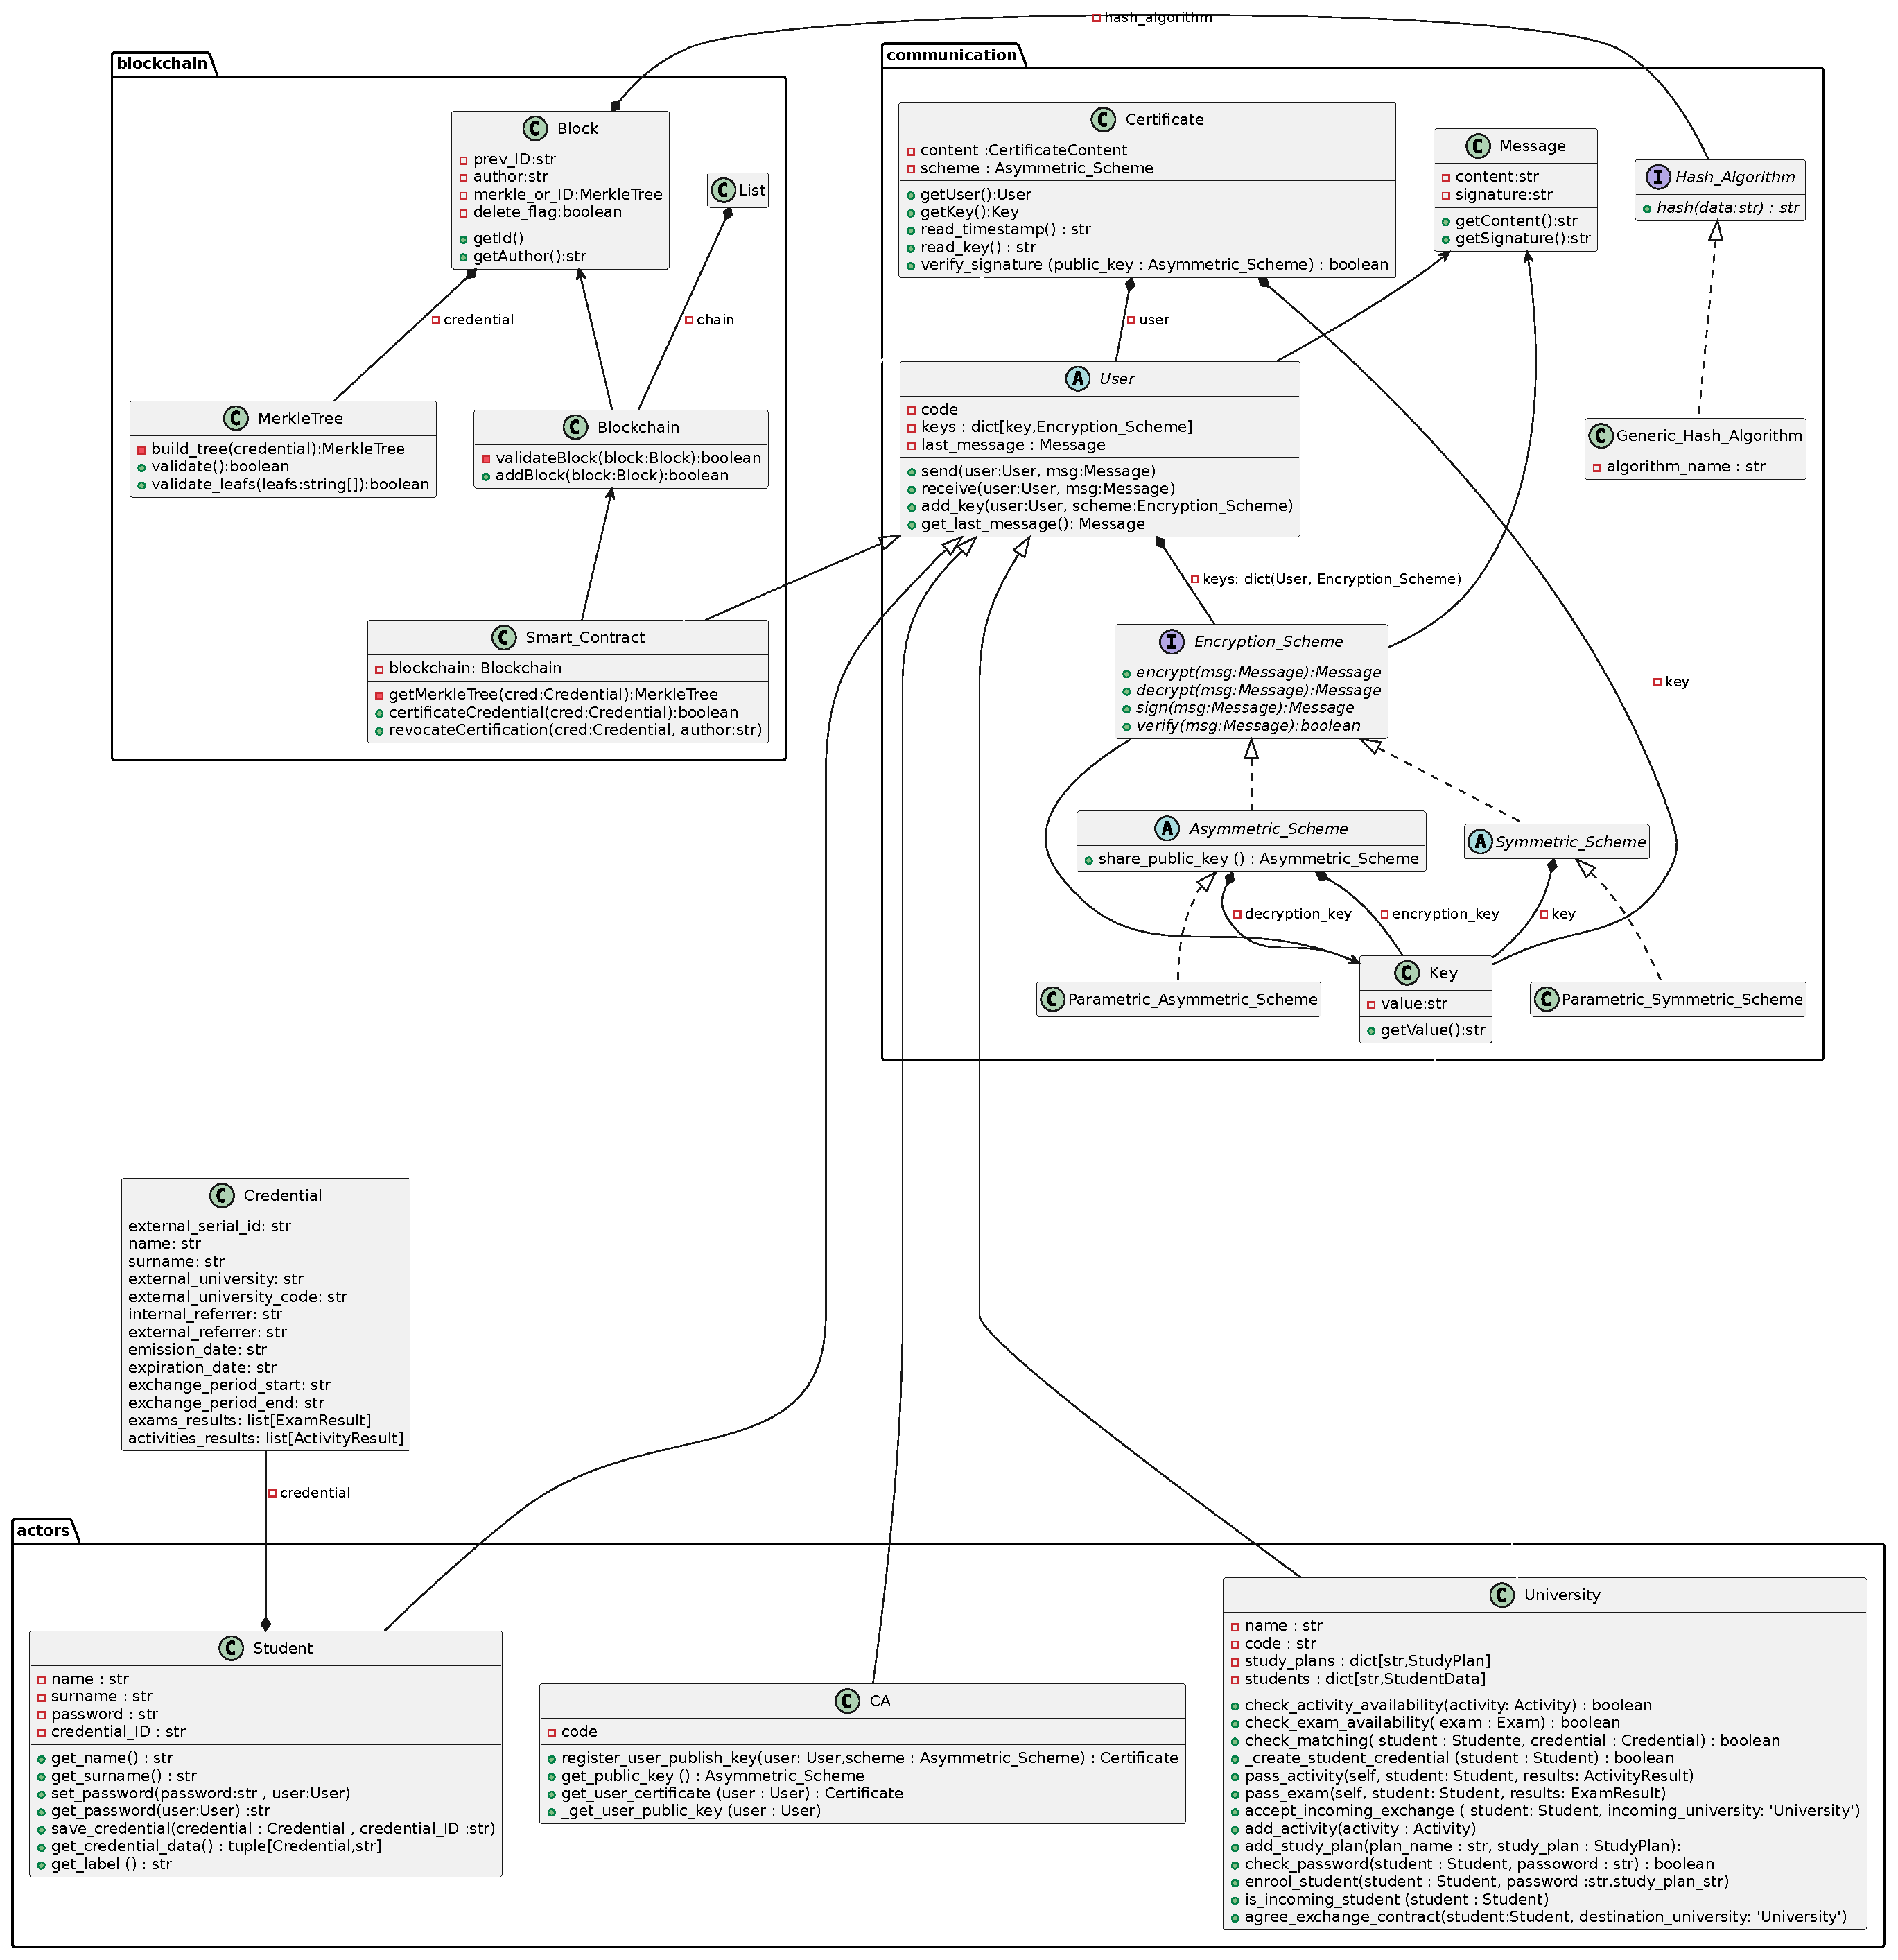
\includegraphics[width=1\textwidth]{uml_design.eps}
    \caption{UML Class Design}
    \label{fig:class_design}
\end{figure}

\subsection{Struttura implementazione}
L'implementazione è suddivisa in diversi algoritmi, ciascuno dei quali collabora con gli altri, nel senso che produce dei risultati che possono essere utilizzati dagli altri algoritmi, ma opera in un contesto proprio, indipendente dagli altri.
\\[1em]
Ogni algoritmo effettua una determinata azione tra quelle descritte nel documento, simulando l'operato di uno o più università, studenti o enti di accreditamento. Le misure di sicurezza adottate in fase di progettazione vengono qui implementate attraverso algoritmi che possono essere parametrizzati sulla base del livello di sicurezza desiderato, e ne vengono misurate le tempistiche.
\\
La suddivisione della logica del progetto in algoritmi permette di testare singolarmente ciascuno di essi, e di verificare che il risultato ottenuto sia quello atteso. Inoltre, la modularità del codice permette di sostituire un algoritmo con uno più efficiente, senza dover modificare il resto del codice.
\\[1em] Gli algoritmi principali, nel quale è distribuito il progetto, sono a loro volta suddivisi in base agli attori principali, eventualmente iniziatori dell'azione descritta mediante tale algoritmo.
\subsection{Parametri di sicurezza}
I parametri di sicurezza vengono utilizzati per configurare gli algoritmi di sicurezza utilizzati, in particolare vanno a influenzare le prestazioni e la sicurezza offerta dagli schemi crittografici e dagli algoritmi di hash. Anche le distribuzioni casuali e la dimensione massima dalle quali vengono presi i nonce vengono parametrizzati in base al livello di sicurezza desiderato. I parametri più importanti sono inseriti nel file \texttt{constants.py}, e sono:
\begin{itemize}
    \item \texttt{SYMMETRIC\_KEY\_LENGTH}: La lunghezza della chiave simmetrica in byte, utilizzata una volta che lo studente si è autenticato con l'università. Questo schema viene utilizzato solo per la durata della sessione, e attraverso questa viene effettuata la cifratura della credenziale inviata dall'università ospitante.
    \item \texttt{IV\_SIZE}: La dimensione del vettore di inizializzazione (IV) in byte, utilizzato negli algoritmi di crittografia simmetrica.
    \item \texttt{MAC\_SIZE}: La lunghezza del codice di autenticazione del messaggio (MAC) in byte, utilizzato per garantire l'integrità dei messaggi cifrati.
    \item \texttt{ASYMMETRIC\_KEY\_LENGTH}: La lunghezza della chiave asimmetrica in byte, utilizzata per la cifratura dei messaggi tra lo studente e le università prima dell'autenticazione. Viene utilizzata per cifrare la chiave simmetrica, e tra le università per firmare e/o cifrare i messaggi. Nel seguente progetto non vi è differenza del tempo di cifratura rispetto all'università e agli studenti, tuttavia sarebbe possibile inserire un ritardo inversamente proporzionale alla potenza computazionale dell'autore del messaggio, per rappresentare questa criticità.
    \item \texttt{EXTRACT\_RANDOM\_NUMBER}: Funzione per estrarre un numero casuale minore di un dato numero definibile come parametro. Utilizzata per generare nonce e le chiavi per gli schemi crittografici. Il numero casuale viene generato attraverso la libreria \texttt{secrets}.
    \item \texttt{MAXIMUM\_TIMESTAMP\_DIFFERENCE}: La differenza massima tra i timestamp accettata per un messaggio, in secondi. Utilizzata per verificare la freschezza dei messaggi tra lo studente e l'università, per rilevare i replay attack.
    \item \texttt{BLOCKCHAIN\_HASH\_ALGORITHM}: L'algoritmo di hash utilizzato per calcolare gli hash. Viene usato per calcolare l'hash delle componenti delle credenziali, dei blocchi, e per comodità il suo uso è esteso alle università per calcolare l'hash delle password, il cui salt è, a solo scopo didattico, una concatenazione del nome e del cognome dello studente. Nel progetto è parametrizzato con \texttt{"SHA256"}.
    \item \texttt{CREDENTIAL\_PERIOD\_DAYS} La durata in giorni di una credenziale dopo che viene emessa, di default. Dopo questi, la credenziale viene considerata scaduta, e non può più essere utilizzata.
    \item \texttt{BLACKLIST\_THRESHOLD} Il rapporto di università rispetto al totale necessario per estromettere una università dal sistema. Quando una università viene estromessa, non è più in grado di interagire con lo smart contract. 
\end{itemize}
Non esiste una combinazione perfetta dei seguenti parametri: la combinazione migliore è frutto del compromesso tra la sicurezza del sistema rispetto alla sua velocità, relativamente alle chiavi, e alla sua reattività rispetto alla manipolabilità relativamente al rapporto di università necessarie per estrometterne una, dalla blockchain o dalle CA, quando implementata tale funzionalità
\subsection{Studente}
\subsubsection{Immatricolazione}
L'algoritmo prende in ingresso le informazioni riguardanti lo studente, l'università e il piano di studi, e simula la procedura d'iscrizione di uno studente presso un'università. Questa procedura richiede quindi che lo studente venga in possesso di un certificato dell'università, attraverso un ente di accreditamento, e che l'università ne registri nome utente e password in un database locale, in modo da poterne verificare l'identità dello studente durante il processo di autenticazione. È compito dell'università inoltre aprire un fascicolo dello studente, nel quale vengono conservate le informazioni concernenti la carriera dello studente.
\\[1em]
In particolare, se lo studente si iscrive all'università ospitante, non è richiesto il piano di studi desiderato, siccome è compito dello studente proporre un piano all'università di origine.
\subsubsection{Autenticazione}
L'algoritmo prende in ingresso lo studente, e simula la procedura di autenticazione dello studente presso un'università. Essa richiede che lo studente sia in possesso di un certificato dell'università, e che l'università ne verifichi l'identità attraverso le credenziali fornitele confrontandole con quelle conservate nel database locale. Questo algoritmo viene usato anche da altri algoritmi per simulare l'autenticazione dello studente presso l'università ospitante, siccome dopo questa procedura sia lo studente che l'università possono comunicare attraverso uno schema crittografico simmetrico.
\subsubsection{Presentazione domanda per accesso a periodo di mobilità}
L'algoritmo prende in ingresso lo studente, e simula la procedura di presentazione della domanda per accedere a un periodo di mobilità. Questa richiede che lo studente sia in possesso di un certificato dell'università di origine, delle credenziali di accesso e di un piano di studi da proporre. Una volta che lo studente si è autenticato e le ha comunicate, citando anche l'università di destinazione alla quale è interessato, l'università di origine procede con l'accettazione o il rifiuto della domanda. L'università di origine, per accertarsi che sia possibile rispettare il piano, comunica con l'università ospitante, attraverso lo schema asimmetrico a loro disposizione. 
\\[1em]
In caso di esito positivo, l'università di origine deve inserire nel proprio fascicolo dello studente le informazioni sul periodo di mobilità, quali le attività accademiche da sostenere e l'università presso cui si svolgerà.
\subsection{Università}
\subsubsection{Registrazione}
L'algoritmo prende in ingresso le informazioni riguardanti l'università, e simula la procedura di registrazione di un'università presso un ente di accreditamento. Questa procedura spesso avviene mediante canali sicuri alternativi, o persino di persona, per cui non vi sono particolari misure di sicurezza individuabili, se non la lunghezza della coppia di chiavi adottata dall'ente di accreditamento per produrre i certificati delle università. Dopo questa procedura, l'università è in possesso di una coppia di chiavi, e gli studenti possono ottenere la chiave pubblica dell'università contattando la CA presso cui si è registrata.
\subsection{Di progetto}
Gli algoritmi qui presentati riguardano la logica interna del progetto e sono utilizzati per simulare le operazioni nelle quali tutti, o quasi tutti, gli attori devono collaborare per raggiungere il risultato desiderato. 
\subsubsection{Emissione \& certificazione credenziale}
L'algoritmo prende in ingresso lo studente e l'università ospitante presso cui sta svolgendo il suo periodo di mobilità, e simula la procedura di emissione della credenziale da parte dell'università ospitante, e la certificazione della stessa. L'università per prima cosa produce la credenziale utilizzando i dati dello studente, sia quelli ottenuti durante la presentazione della domanda del periodo di mobilità che quelli prodotti durante la carriera nell'università. Prodotta la credenziale, suddivide la credenziale in vari blocchi: in uno inserisce i dati generici della credenziale, per ciascun esame genera un blocco, e per ciascuna attività ne genera altri. In ciascun blocco è presente un dizionario di informazioni, e lo usa per ottenere prima una forma in stringa, e poi l'hash attraverso l'algoritmo condiviso dalle università. Una volta ottenuta la lista degli hash, ciascuno calcolato su un blocco, la comunica allo smart contract della blockchain, il quale provvede a generare un Merkle Tree le cui foglie sono i blocchi hashati forniti dall'università. Ottenuto il Merkle Tree, lo smart contract genera un nuovo blocco nella blockchain, contenente:
\begin{itemize}
    \item L'ID del blocco precedente, o l'hash di "Genesis Block" se è il primo
    \item L'hash della chiave pubblica dell'università che ha emesso la credenziale
    \item La delete flag, pari a 0 in questo caso
    \item Il Merkle Tree generato
    \item L'ID come hash del contenuto del blocco
\end{itemize}
Il blocco viene quindi inserito nella blockchain, e lo smart contract ne restituisce l'ID all'università ospitante, la quale lo inoltra allo studente, che lo comunicherà con la università di origine.
\subsubsection{Presentazione \& validazione credenziale}
L'algoritmo prende in ingresso lo studente e l'università di origine, e simula la procedura di presentazione della credenziale da parte dello studente all'università di origine, e la validazione della stessa. Prima di tutto, lo studente deve decidere quali informazioni rimuovere dalla credenziale attraverso la divulgazione selettiva, che consiste nel rimuovere le parti della credenziale che contengono informazioni superflue. Una volta che lo studente ha deciso, comunica la credenziale ottenuta e l'ID all'università, previa autenticazione. L'università procede a controllare se la credenziale è in linea con quella che si attendeva dallo studente: se la data della credenziale è valida, se contiene tutti gli esami richiesti, e se fa riferimento allo studente. Una volta fatto questa verifica, deve interrogare lo smart contract attraverso sia l'ID fornito, che la forma in blocchi hashati della credenziale. Lo smart contract cercherà nella blockchain un blocco con lo stesso ID:
\begin{itemize}
    \item Se la ricerca va a buon fine, deve controllare che tutti gli hash dei blocchi della credenziale appartengano alle foglie del Merkle Tree contenuto nel blocco. L'associazione dev'essere uno ad uno. Ciò significa che la credenziale è stata certificata. Tuttavia, è necessario controllare che non sia stata revocata scorrendo il resto della blockchain.
    \item Se la ricerca non va a buon fine o l'albero non contiene tutti gli hash tra le foglie, significa che la credenziale non esiste oppure è stata manomessa.
\end{itemize}
Lo smart contract provvede quindi a comunicare l'esito all'università.
\subsubsection{Revoca della credenziale}
L'algoritmo prende in ingresso lo studente e l'università ospitante, e simula la procedura di revoca della credenziale da parte dell'università ospitante. Prima di tutto, l'università deve comunicare allo smart contract l'ID della credenziale da revocare. Lo smart contract a sua volta cerca nella blockchain se il blocco esiste, in caso positivo, controlla allora che non sia stato già revocato. Quando arriva alla fine della blockchain significa che deve aggiungere un nuovo blocco che invalidi quello contenente la credenziale. Crea quindi alla fine un nuovo blocco, contenente:
\begin{itemize}
    \item L'ID del blocco precedente
    \item L'hash della chiave pubblica dell'università che ha emesso la credenziale
    \item La delete flag, pari a 1 in questo caso
    \item L'ID della credenziale, corrispondente al blocco revocato
    \item L'ID come hash del contenuto del blocco
\end{itemize}
Quando si vuole controllare che la credenziale non sia stata revocata, è sufficiente scorrere la blockchain e controllare che, nei blocchi revocatori, non ci sia l'ID della credenziale.
\subsubsection{Algoritmi di cifratura e decifratura}
Rispetto agli altri algoritmi, questi non vengono utilizzati per simulare le operazioni effettuate dagli attori, ma per permetterle. Gli algoritmi di sicurezza vengono valutati sulla base delle prestazioni in termini di tempo, e sicurezza offerta, in base ai parametri di sicurezza configurati.
\\[1em]
La valutazione delle prestazioni sulla base del tempo che essi impiegano è di vitale importanza, siccome permette il confronto tra implementazioni e la scelta che, contestualizzata in merito al seguente progetto, risulta essere la migliore.
\subsection{Tecnici}
\subsubsection{Rimozione dei file salvati}
Questa funzionalità è utile per formattare lo stato del progetto e riportarlo alle condizioni originali, siano essi relativi alla logica degli attori, oppure relativi alle esecuzioni, ai risultati e così via.
\subsubsection{Modifica dei parametri di sicurezza}
Qui è possibile manipolare i vari parametri necessari agli algoritmi per funzionare, come la lunghezza delle chiavi, le funzioni di hash utilizzate e altri aspetti crittografici. La loro inizializzazione è contenuta all'interno del file \texttt{constants.py}.
\subsubsection{Visualizzazione dei tempi di esecuzione}
Per ciascun algoritmo vengono valutati i tempi di esecuzione, e mostrati alla fine dell'esecuzione.
\subsection{Simulazione degli attacchi}
Questi algoritmi simulano gli attacchi descritti nella sezione del WP3, mostrandone le conseguenze e le eventuali contromisure adottate dal sistema.
\subsubsection{Violazione dell'ente di accreditamento}
Il seguente algoritmo simula la violazione di un ente di accreditamento, gli effetti di questo attacco sono stati già descritti nel WP3, e per l'assenza di contromisure, non è possibile difendersi. Tuttavia, è presente per completezza.
\subsubsection{Violazione dell'università ospitante}
L'algoritmo simula la violazione di una università ospitante, la contromisura adottata dal sistema è quella di estrometterla dalla blockchain: delle altre università votano, attraverso lo smart contract, l'estromissione. Se la quota dei voti supera la soglia richiesta, verrà impedito all'università di accedere alla blockchain per certificare credenziali.
\subsubsection{Violazione dell'università di origine}
Similmente all'algoritmo precedente, simula la violazione dell'università di origine. Allo stesso modo nuove università votano l'estromissione, in caso di superamento della soglia tale università non sarà più in grado di usufruire dei servizi della blockchain.
\subsubsection{Studente malevolo}
Il seguente algoritmo simula uno studente malevolo, intenzionato a divulgare informazioni false riguardo la sua credenziale. L'algoritmo mostra cosa accade quando uno studente altera i campi della credenziale, il caso in esame preso è quello dove viene aggiunto un esame agli esiti della credenziale. L'università, quando invia la lista dei blocchi hashati delle componenti della credenziale alterata allo smart contract, questi si accorge dell'alterazione, siccome ad un blocco della credenziale non corrisponde alcuna foglia del Merkle Tree.
\subsubsection{Intercettatore di comunicazioni dell'università ospitante}
Questo algoritmo simula la presenza di un intercettatore tra la comunicazione con l'università ospitante e lo studente. In particolare, lo scenario in esame è preso durante la fase di immatricolazione. Quando lo studente apre la comunicazione con l'università e chiede di autenticarsi, comunica il primo numero casuale che genera. L'attaccante non lo può conoscere, ma conosce il momento nel quale ha generato il primo e il secondo numero casuale. Quando l'università risponde, espone il primo numero casuale, per cui l'attaccante potrebbe tentare di inferire il secondo numero casuale, conoscendo il primo.
\\[1em]
Tale attacco è possibile nel momento in cui lo studente sta per inviare la password con la quale registrarsi all'università: se l'attaccante modifica il messaggio, potrebbe riempire tutti i campi, ma non conoscerebbe solamente il nonce casuale da inserire al messaggio. Per questa ragione, intercetta il messaggio, lo cancella e ne inietta un altro con le stesse informazioni, ma un nonce eventualmente diverso e una password diversa, conosciuta da lui solamente. La probabilità che questo attacco abbia successo è inversamente proporzionale alla sicurezza del generatore di numeri (pseudo)casuali e la dimensione massima del numero casuale.
\subsubsection{Attacco con credenziale nota}
In questo attacco si simula un attaccante che conosce la credenziale dello studente, e tenta di inferire informazioni o quanto meno compromettere il sistema. Tuttavia, siccome la comunicazione della credenziale da parte dell'università ospitante avviene in un schema crittografico simmetrico, e il messaggio contiene inoltre il timestamp, e l'ID che l'attaccante potrebbe non conoscere, non gli è possibile alterare la credenziale senza destare sospetto. Difatti, se l'alterasse durante l'emissione, lo studente noterebbe la compromissione dell'integrità, viceversa durante la presentazione della credenziale, la noterebbe l'università di origine.
\subsubsection{Divulgazione di informazioni superflue}
In questo algoritmo si simula la divulgazione di informazioni superflue da parte dello studente, che decide di inviare all'università di origine una credenziale con informazioni non necessarie. Tuttavia, siccome il sistema non ha alcun controllo su ciò che lo studente decide di divulgare, non è possibile impedire tale operazione. L'unica soluzione sarebbe di proporre allo studente un'applicativo che, ottenuto il piano di studi in mobilità proposto, effettui il filtraggio delle informazioni superflue. In questo modo, lo studente non potrebbe divulgare informazioni superflue, siccome l'applicazione non glielo consentirebbe.
\subsection{Moduli}
L'implementazione del progetto è suddivisa in moduli, ciascun modulo ha una finalità e responsabilità ben delineate. 
\subsubsection{Modulo di comunicazione}

È il modulo che implementa in maniera astratta la comunicazione tra gli attori del sistema, gli attori del sistema sono rappresentati dalle rispettive classi, che implementano la classe astratta \texttt{User}.
Inoltre, il modulo permette la gestione delle chiavi associate agli utenti sfruttando la classe \texttt{Key}.
\\[1em]
Le classi \texttt{Parametric Asymmetric Scheme} e \texttt{Parametric Symmetric Scheme} sono basate su un'interfaccia comune fornita dalla classe \texttt{Encryption Scheme}, garantendo l'interazione tra gli attori del sistema mediante l'interfaccia comune.
Le classi concrete permettono inoltre di effettuare modifiche ai parametri di sicurezza utilizzati dagli schemi, garantendo estendibilità e manutenibilità del codice per sviluppi futuri. La logica di entrambi gli schemi sono stati implementati con l'utilizzo della libreria \texttt{cryptography}.
\\[1em]
La classe \texttt{Generic Hash Algorithm} permette di decidere quale algoritmo di hashing utilizzare e fornisce i metodi per calcolare l'hash dei dati, sfruttando la libreria \texttt{hashlib}. 

\subsubsection{Modulo blockchain}
Il modulo implementa la logica di funzionamento della blockchain, in particolare nella classe \texttt{Blockchain} è presente la struttura dati che gestisce la lista dei blocchi, la cui implementazione di ciascuno è fornita dalla classe \texttt{Block}. 
\\[1em]
La classe \texttt{Smart Contract} sovrintende la gestione della blockchain. È presente un'implementazione personalizzata di \texttt{MerkleTree}, che gestisce la creazione della omonima struttura, seguendo la logica di funzionamento nota.

\subsubsection{Modulo attori}
Il modulo attori fornisce delle implementazioni concrete della classe \texttt{User}: 
la classe \texttt{Student} che memorizza le credenziali e le password per le diverse università, create durante l'esecuzione della funzione immatricolazione. 
\\[1em]
La classe \texttt{University} che modella un ateneo, gli attributi più rilevanti sono piano di studi, attività e un registro contenente gli studenti iscritti. 
Le sue principali responsabilità sono la gestione degli studenti e i relativi esami, e l'interazione con lo smart contract. 
\\[1em]
La classe \texttt{CA}, rappresenta la Certification Authority e tramite i suoi metodi permette di registrare un utente tramite la sua chiave pubblica contestualmente rilasciando un certificato contenente la chiave registrata.
\subsection{Esempio di esecuzione in \texttt{main.py}}
Nella cartella principale è stato creato un file \texttt{main.py} che funge da entry point del progetto, e permette di eseguire gli algoritmi implementati. Il flusso di esecuzione si divide in tre parti, in base all'ingresso che viene immediatamente fornito dopo l'esecuzione:
\begin{itemize}
    \item Se si inserisce la lettera 'C' è possibile eseguire uno degli algoritmi sopracitati che riguarda il funzionamento del sistema. Ciascun algoritmo chiederà all'utente di inserire i valori necessari al suo corretto funzionamento.
    \item Se si inserisce la lettera 'H' è possibile eseguire una configurazione predefinita (ma ancora configurabile) del codice proposta dagli autori del progetto. Tale configurazione rappresenta il caso proposto nella traccia del progetto, contente:
    \begin{itemize}
        \item Una singola CA a cui sia le università che gli studenti fanno riferimento
        \item Uno studente
        \item Una università di origine, alla quale lo studente è immatricolato
        \item Una università ospitante, dove la quale lo studente desidera effettuare il suo periodo di mobilità
    \end{itemize}
    Questa esecuzione prevede l'esecuzione di tutti quanti gli algoritmi mostrati, con ingressi predefiniti. A ciascun algoritmo l'esecuzione si ferma e descrive a terminale una breve introduzione di ciò che sta avvenendo.
    \item Se si inserisce la lettera 'A' è possibile lanciare l'esecuzione predefinita in modalità di analisi delle prestazioni temporali, questa configurazione risulta estremamente utile quando si voglio valutare le prestazioni temporali in funzione dei parametri di sicurezza. Alla fine dell'esecuzione, il codice mostra un report contenenti i tempi di esecuzione per gli algoritmi principali, e per validazione, emissione e certificazione della credenziale.
\end{itemize}
\subsection{Simulazioni degli attacchi in \texttt{simulate\_attack.py}}
All'interno del file \texttt{simulate\_attack.py} sono presenti i diversi algoritmi che permettono di simulare attacchi al sistema. Essi possono essere richiamati per mostrare le conseguenze e le eventuali contromisure adottate dal sistema. La loro esecuzione è guidata e stampano a terminale l'eventuale eccezione qualora l'attacco fallisse.
\end{document}